\documentclass{article}
\usepackage[utf8]{inputenc}

\title{Problem Set 10}
\author{Mason Ross Hayes}
\date{7 April 2020}

\usepackage{natbib}
\usepackage{graphicx}
\usepackage{hyperref}


\begin{document}


\maketitle

\section{Tuned Parameters}

I could not figure out how to get SVM and glmnet to work in mlr3. It returned error that "factor" wasn't a supported feature for these models.
I also could not get nnet to work in mlr3. All of these worked in mlr, but in this Problem Set I report only results from mlr3.

For the tree model: 

Tuned x: cp=0.04477, minsplit = 16, minbucket = 31, F1 = 0.8958 

For KKNN, K = 28. 

Naive bayes actually outperformed both the tree and kknn models.



\begin{figure}
    \centering
    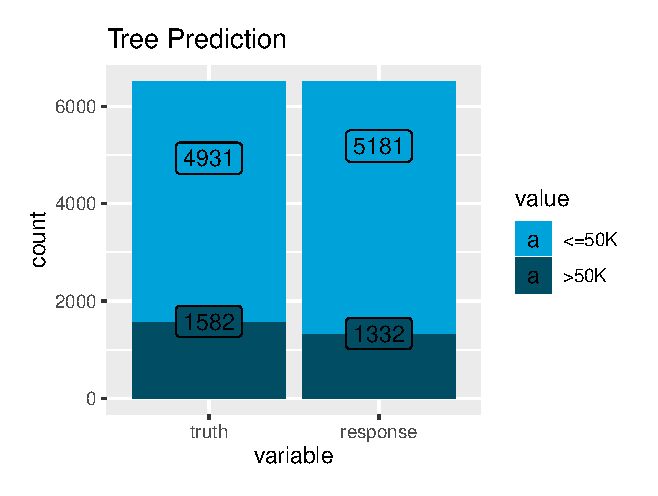
\includegraphics{tree_prediction.eps}
    \caption{N = 6513}
    \label{fig:my_label}
\end{figure}

\begin{figure}
    \centering
    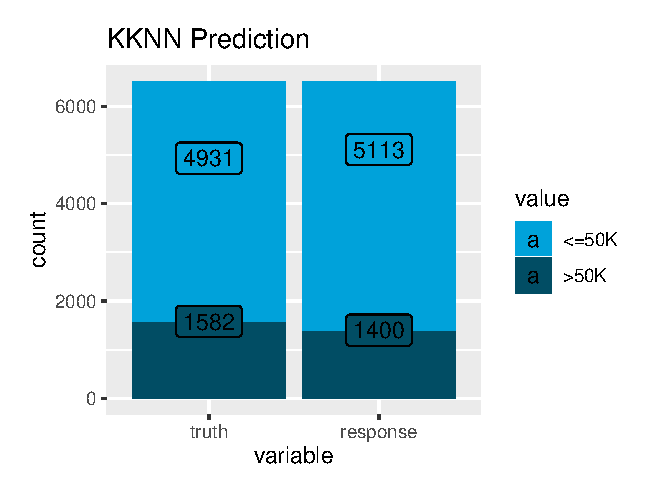
\includegraphics{kknn_prediction.eps}
    \caption{N = 6513}
    \label{fig:my_label}
\end{figure}

\begin{figure}
    \centering
    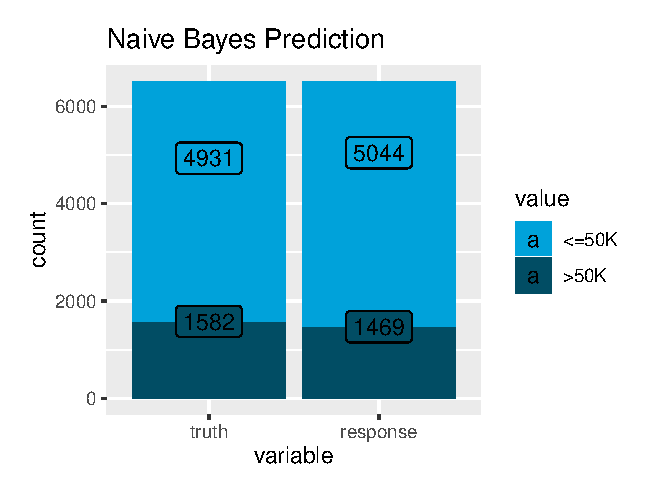
\includegraphics{bayes_prediction.eps}
    \caption{N = 6513}
    \label{fig:my_label}
\end{figure}

\end{document}